\documentclass{article}
\usepackage{graphicx}

\providecommand{\floor}[1]{\left \lfloor #1 \right \rfloor}

\title{\textbf{2025 Parallel and Distributed Computing Assignment \#2}}
\date{May 4, 2025}
\author{Doyoung Kim}

\begin{document}
\maketitle

This assignment focuses on implementing a shared-memory parallel program that 
performs LU decomposition using pthreads. We also compare the pthread version 
with the OpenMP implementation in terms of execution time and parallel efficiency.

Pthreads (POSIX threads) provide a standardized API for multithreaded 
programming. The interface defines fundamental operations such as thread 
creation and termination (\verb|pthread_create()|, \verb|pthread_exit()|), as 
well as synchronization primitives like mutexes and condition variables. Because 
pthreads are language- and architecture-independent, they allow developers to 
write portable and efficient parallel programs.

\section{Implementation}

This section describes the pthread version of the LU decomposition routine, 
specifically \verb|lu_decomposition_parallel()|. The other routines are largely 
similar to the previous version, except that matrices are now represented as 
vectors of vectors. Minor modifications were also made to 
\verb|lu_decomposition_omp()| to eliminate potential race conditions and 
conform to the updated function prototype provided in the skeleton code.

The \verb|lu_decomposition_parallel()| routine is executed by the master thread. 
It begins by initializing the permutation vector and copying the target matrix 
\verb|A|. It also sets up global variables and barriers to be shared among 
worker threads. The master thread then spawns worker threads using 
\verb|pthread_create()|.

In addition to coordination, the master thread is responsible for completing the 
"residual loops"—the portions of iterations not evenly distributed among worker 
threads. If there are $t$ worker threads and a loop that executes $n$ times, 
each worker is assigned $\floor{\frac{n}{t}}$ iterations. This leaves 
$n - \floor{\frac{n}{t}} \times t$ residual iterations, which the master thread 
handles. The master thread also waits for all worker threads to finish before 
proceeding.

In each top-level loop (over \verb|k|), the master thread performs the following 
steps:

1. Pivot selection: It finds the pivot row within the current matrix block. 
This step must be done sequentially to avoid race conditions on the pivot 
variable. After identifying the pivot, the master swaps it with the first row of 
the block and updates \verb|U[k][k]| with the first element of the pivot row.

2. Residual update: The master waits for the worker threads to compute their 
loop bounds. Once confirmed, it executes the residual loop iterations for 
updating the lower (\verb|L|) and upper (\verb|U|) triangular matrices.

3. Matrix update: After the worker threads update their respective portions 
of \verb|L| and \verb|U|, the master completes the remaining updates to the 
target matrix.

Worker threads perform similar operations, excluding the pivot selection. For 
each top-level loop, a worker thread calculates its loop bounds based on its t
hread ID, the total number of threads, and the loop size. After completing its 
portion of the update, it waits for other threads to finish and then updates its 
designated portion of the target matrix.

Synchronization is managed using three barriers: \verb|barrier1|, 
\verb|barrier2|, and \verb|barrier3|. Shared data—including the target matrix, 
\verb|L|, \verb|U|, number of threads, and matrix size—is maintained as global 
variables.

\section{Efficiency}

Execution time was measured using \verb|std::chrono::steady_clock|. The time 
required to generate the input matrix, initialize the output matrices, and 
verify the result was excluded from the measurements. Tests were conducted on a 
MacBook Pro M3 (11-core model) with 18 GiB of unified memory, running a Docker 
container based on the Ubuntu 24.04 image. Each configuration was executed five 
times, and the reported results are averages.

\begin{figure}[h]
\centering
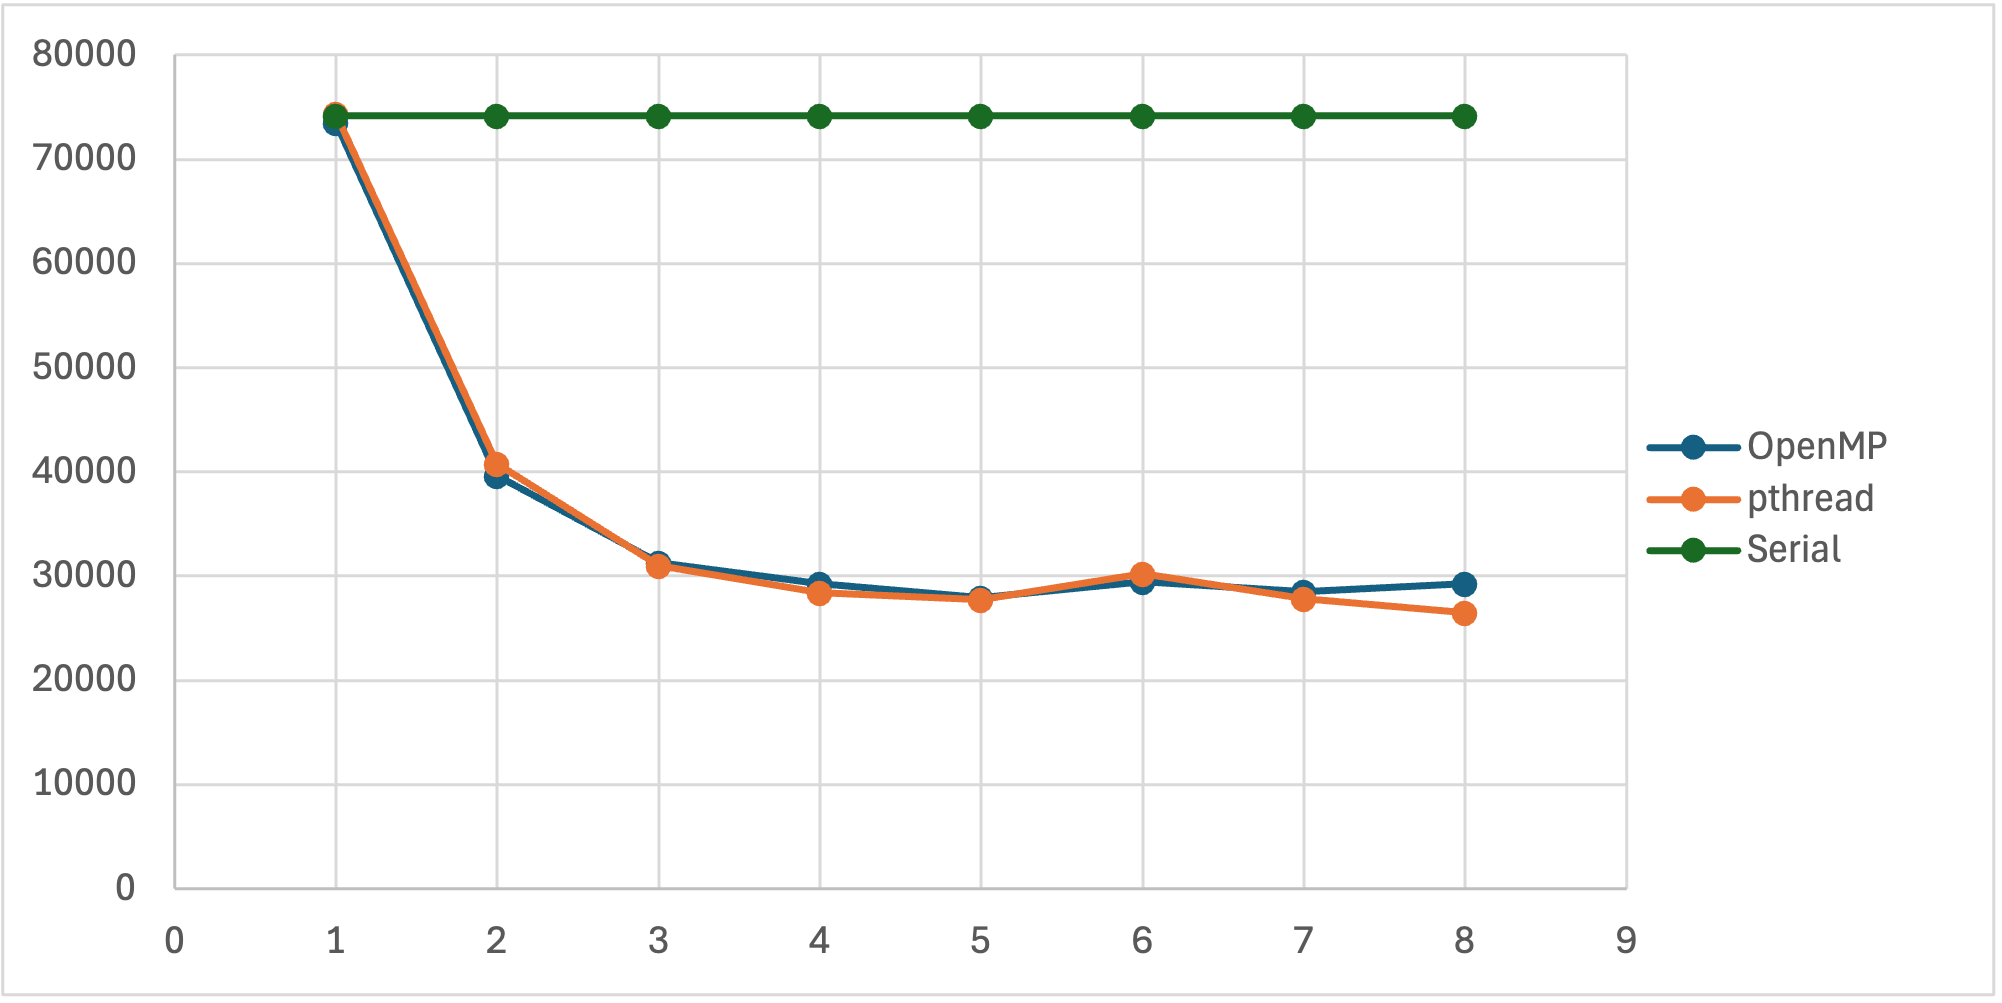
\includegraphics[width=.75\textwidth]{figure1.png}
\caption{
    Execution time of LU decomposition using pthreads and OpenMP, with varying 
    thread counts. The X-axis represents the number of threads; the Y-axis shows 
    execution time in milliseconds. The horizontal line indicates the execution 
    time of the serial version.
}
\end{figure}

Figure 1 shows that execution time generally decreases as the number of threads 
increases, up to a certain point. The pthread and OpenMP version showed almost
identical execution time.

\begin{figure}[h]
\centering
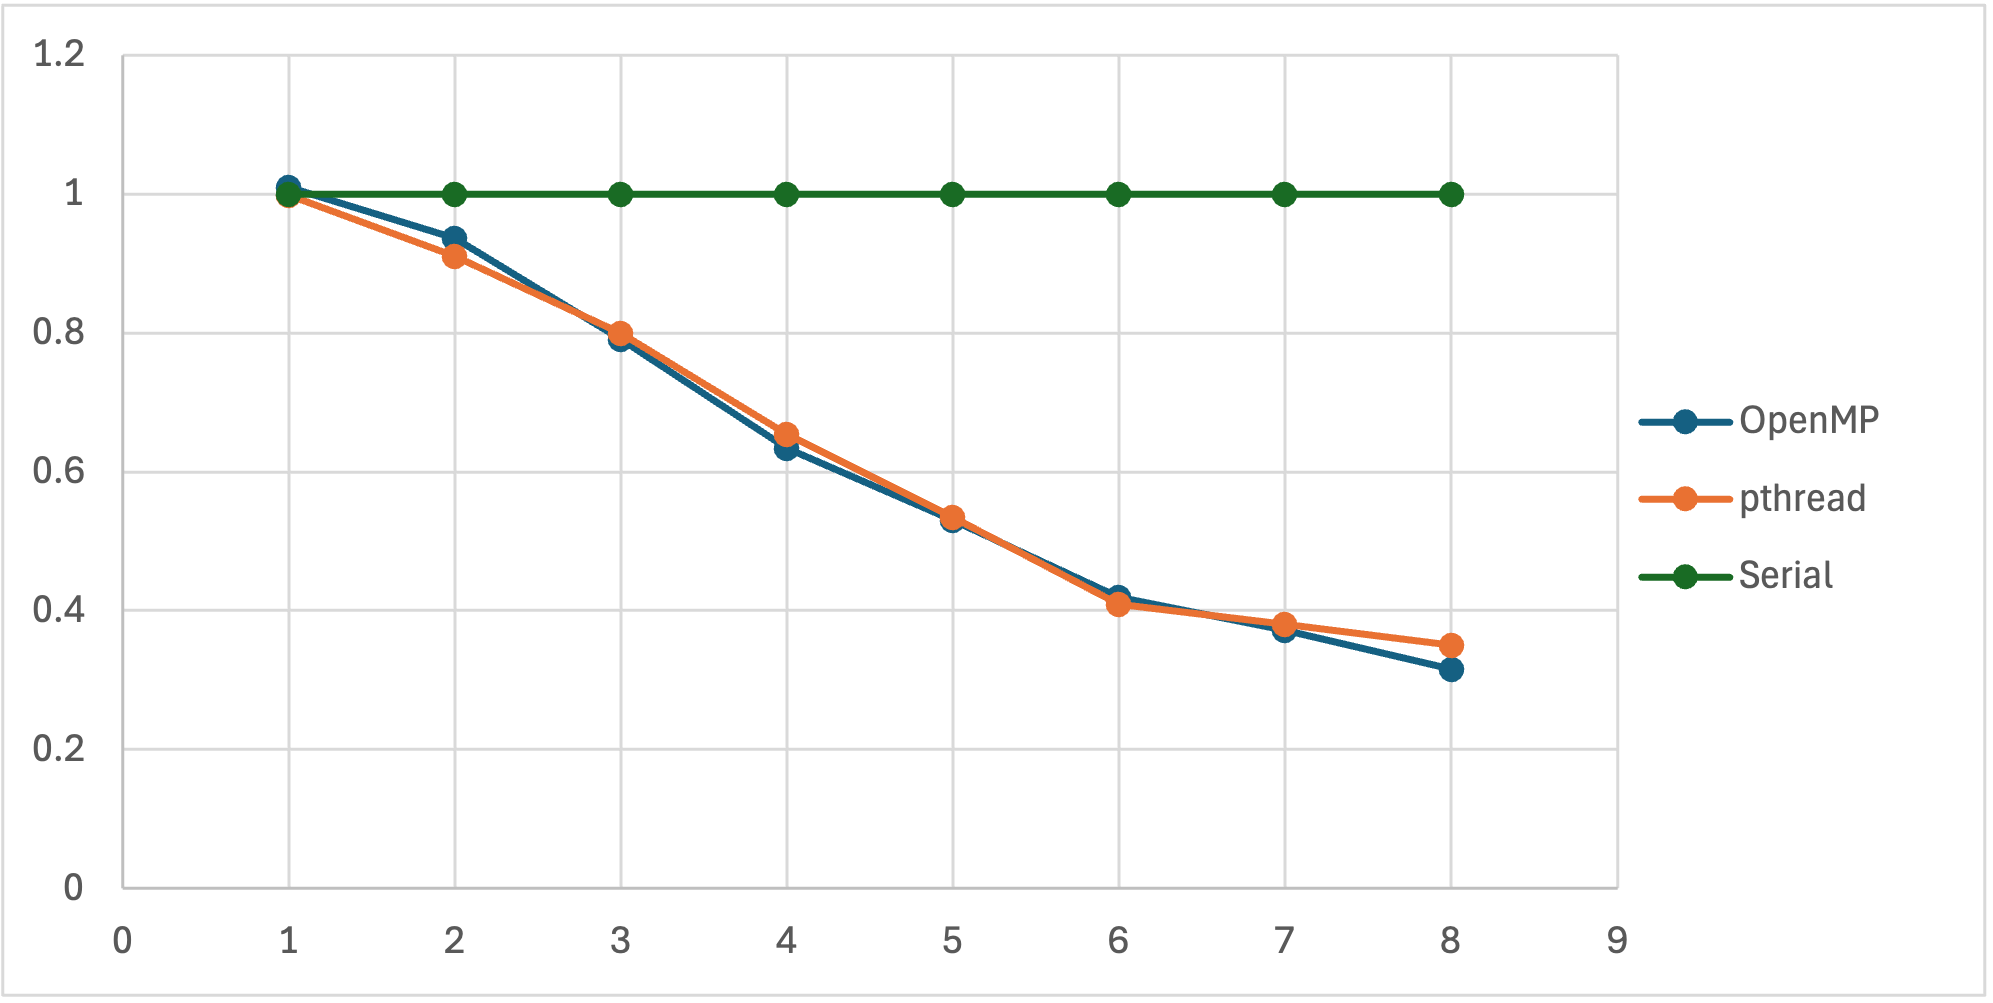
\includegraphics[width=.75\textwidth]{figure2.png}
\caption{
    Parallel efficiency of the pthread and OpenMP implementations. The X-axis 
    represents the number of threads, and the Y-axis shows parallel efficiency, 
    computed as $\frac{S}{pT(p)}$, where $S$ is the serial execution time, $p$ 
    is the number of threads, and $T(p)$ is the parallel execution time.
}
\end{figure}

Figure 2 presents the calculated parallel efficiencies. Since their execution 
time were almost same, they the parallel efficiencies of them were almost 
identical also.

These results suggest that the pthread implementation is generally equally 
efficient with the OpenMP implementation. Although OpenMP’s runtime environment 
automatically distributes loop iterations and manages thread creation and 
synchronization, a programmer can achieve nearly the same level of efficiency 
with pthread. 

\section{Conclusion}

In this assignment, we implemented a shared-memory parallel LU decomposition 
algorithm using pthreads. We evaluated its execution time and parallel 
efficiency, comparing the results with an OpenMP-based implementation. Through 
this work, we gained practical experience with the pthread API and a deeper 
understanding of how low-level thread management affects performance in parallel 
computing.

\end{document}
